\documentclass[
  captions=tableheading,
  bibliography=totoc, 
  titepage=firstiscover,
]{scrartcl}

\usepackage{blindtext} %neuer input

\usepackage{longtable} % Tabellen über mehrere Seiten

\usepackage[utf8]{inputenc} %neuer input

\usepackage{scrhack}

\usepackage[aux]{rerunfilecheck} %Warnung falls nochmal kompiliert werden muss

\usepackage{fontspec} %Fonteinstellungen

\recalctypearea{}

\usepackage[main=ngerman]{babel} %deutsche Spracheinstellung

\usepackage{ragged2e} %neuer input

\usepackage{amsmath, nccmath}

\usepackage{amssymb} %viele mathe Symbole

\usepackage{mathtools} %Erweiterungen für amsmath


\DeclarePairedDelimiter{\abs}{\lvert}{\rvert}
\DeclarePairedDelimiter{\norm}{\lVert}{\rVert}

\DeclarePairedDelimiter{\bra}{\langle}{\rvert}
\DeclarePairedDelimiter{\ket}{\lvert}{\rangle}

\DeclarePairedDelimiterX{\braket}[2]{\langle}{\rangle}{
#1 \delimsize| #2
}

\NewDocumentCommand \dif {m}
{
\mathinner{\symup{d} #1}
}


\usepackage[
  math-style=ISO,
  bold-style=ISO,
  sans-style=italic,
  nabla=upright,
  partial=upright,
  warnings-off={
    mathtools-colon,
    mathtools-overbracket,
  },
]{unicode-math}

\setmathfont{Latin Modern Math}
\setmathfont{XITS Math}[range={scr, bfscr}]
\setmathfont{XITS Math}[range={cal, bfcal}, StylisticSet=1]


\usepackage[
  locale=DE,
  separate-uncertainty=true,
  per-mode=reciprocal,
  output-decimal-marker={,},
]{siunitx}

\usepackage[autostyle]{csquotes} %richtige Anführungszeichen

\usepackage{xfrac}

\usepackage{float}

\floatplacement{figure}{htbp}

\floatplacement{table}{htbp}

\usepackage[ %floats innerhalb einer section halten
  section,   %floats innerhalb er section halten
  below,     %unterhalb der Section aber auf der selben Seite ist ok
]{placeins}

\usepackage[
  labelfont=bf,
  font=small,
  width=0.9\textwidth,
]{caption}

\usepackage{subcaption} %subfigure, subtable, subref

\usepackage{graphicx}

\usepackage{grffile}

\usepackage{booktabs}

\usepackage{microtype} %Verbesserungen am Schriftbild

\usepackage[
backend=biber,
]{biblatex}

\addbibresource{../lit.bib}

\usepackage[ %Hyperlinks im Dokument
  german,
  unicode,
  pdfusetitle,
  pdfcreator={},
  pdfproducer={},
]{hyperref}

\usepackage{bookmark}

\usepackage[shortcuts]{extdash}

%\usepackage{warpcol}

\usepackage{physics}
\allowdisplaybreaks

\begin{document}
    \title{Physik IV Übungsblatt 8}
    \author{  
    Tobias Rücker\\
    \texorpdfstring{\href{mailto:tobias.ruecker@tu-dortmund.de}{tobias.ruecker@tu-dortmund.de}
    \and}{,} 
    Paul Störbrock\\
    \texorpdfstring{\href{mailto:paul.stoerbrock@tu-dortmund.de}{paul.stoerbrock@tu-dortmund.de}}{}
    }
\maketitle
\center{\Large Abgabegruppe: \textbf{4H}}
\thispagestyle{empty}

\newpage
\tableofcontents
\thispagestyle{empty}
\newpage

\setcounter{page}{1}

\section{Aufgabe 1}

    \begin{figure}[H]
        \centering
        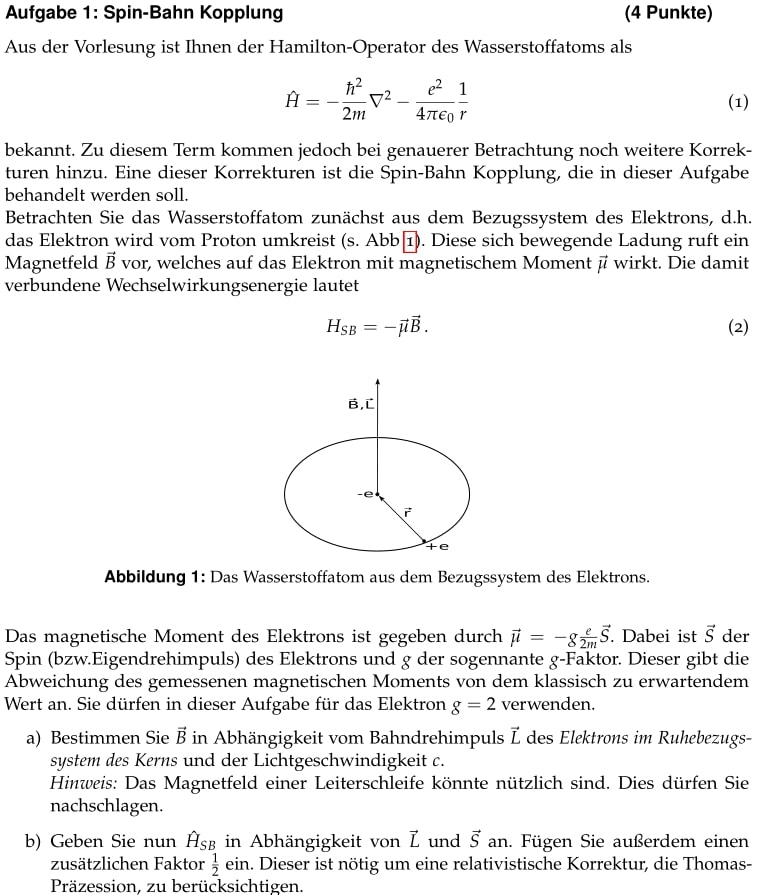
\includegraphics[width=\textwidth]{images/Aufgabe1a.jpg}
        \label{fig:1}
    \end{figure}

    \begin{figure}[H]
        \centering
        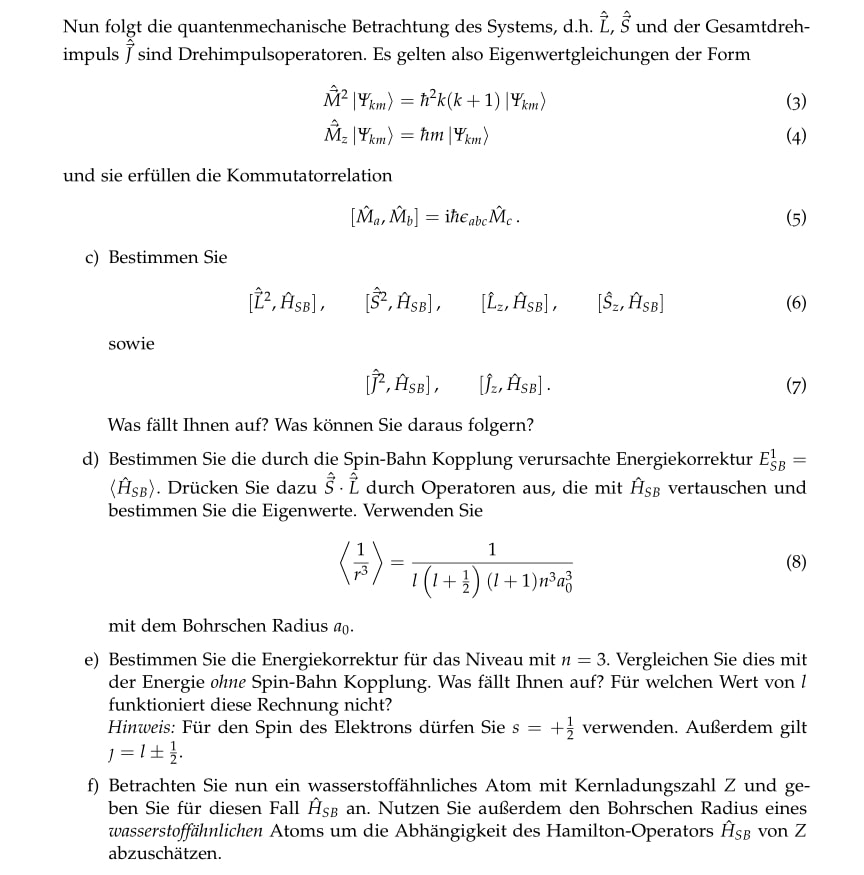
\includegraphics[width=\textwidth]{images/Aufgabe1b.jpg}
        \label{fig:2}
    \end{figure}

    \subsection{a)}

    \subsection{b)}

    \subsection{c)}

    \subsection{d)}

    \subsection{e)}

    \subsection{f)}

\section{Aufgabe 2}

    \begin{figure}[H]
        \centering
        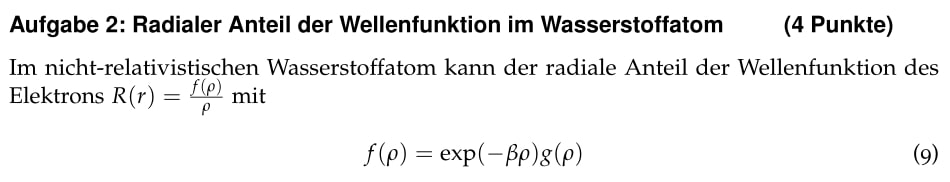
\includegraphics[width=\textwidth]{images/Aufgabe2a.jpg}
        \label{fig:3}
    \end{figure}

    \begin{figure}[H]
        \centering
        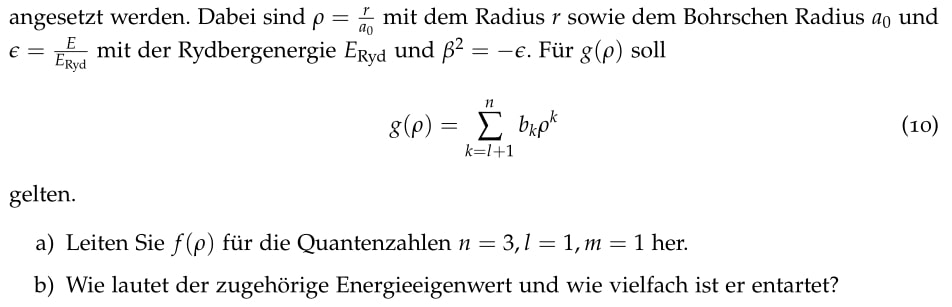
\includegraphics[width=\textwidth]{images/Aufgabe2b.jpg}
        \label{fig:4}
    \end{figure}

    \subsection{a)}

    \begin{align*}
        n &= 3,\;l = m = 1\\
        \\
        \Psi(r,\theta,\varphi) &= R(r)Y(\theta,\varphi)\\
        &= \frac{f(\rho)}{\rho} \sqrt{\frac{2l+1}{4\pi} \frac{(l-m)!}{(l+m)!}} P_l^m(\cos(\theta)) e^{im\varphi}
        \intertext{
            \flushleft{Mit\;}\justifying $P_1^1(\cos(\theta)) = -\sin(\theta)$ folgt:
        }
        &= \frac{f(\rho)}{\rho} \sqrt{\frac{3}{4\pi} \frac{1}{2}} (-\sin(\theta)) e^{i\varphi}
        \intertext{
            \flushleft{Das\;}\justifying $g(\rho)$ des Radialteils ist für $n=3$ und $l=1$ gleich $6\rho^2-\rho^3$. Daraus folgt für $f(\rho)$:
        }
        f(\rho) &= e^{-\beta\rho} \frac{6\rho^2-\rho^3}{\rho} = e^{-\beta\rho} \left( 6\rho-\rho^2 \right)
        \intertext{
            \flushleft{Eingesetzt\;}\justifying ergibt sich für $\Psi$:
        }
        &= e^{-\beta\rho} \left( 6\rho-\rho^2 \right) \sqrt{\frac{3}{8\pi}} (-\sin(\theta)) e^{i\varphi}
    \end{align*}

    \subsection{b)}

    \flushleft{Der\;}\justifying Energieeigenwert lautet
    \begin{align*}
        E &= -E_{Ryd}\frac{1}{n^2} = -E_{Ryd}\frac{1}{9}
        \intertext{
            \flushleft{Für\;}\justifying die Quantenzahl $n=3$ ist die Energie $n^2$-mal, also 9-fach entartet.
        }
    \end{align*}

\section{Aufgabe 3}

    \begin{figure}[H]
        \centering
        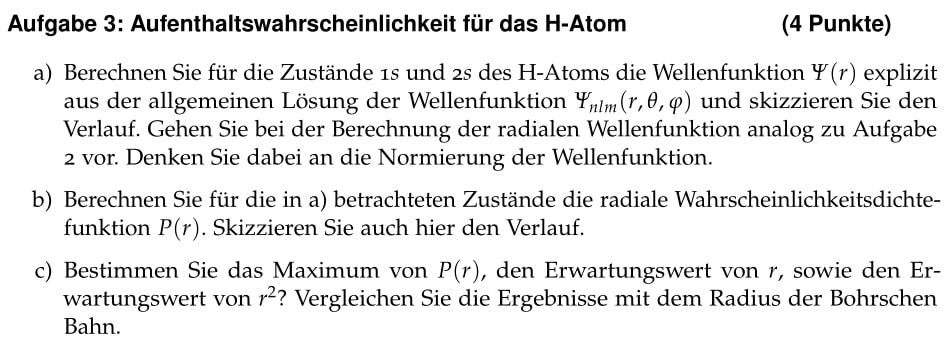
\includegraphics[width=\textwidth]{images/Aufgabe3.jpg}
        \label{fig:5}
    \end{figure}

    \subsection{a)}

    \flushleft{s1:\;}\justifying $n=1, l=m=0$
    \begin{align*}
        \Psi(r,\theta,\varphi) &= \frac{f(\rho)}{\rho} \sqrt{\frac{2l+1}{4\pi} \frac{(l-m)!}{(l+m)!}} P_l^m(\cos(\theta)) e^{im\varphi}
        \intertext{
            \flushleft{Für\;}\justifying $n=1,l=m=0$ ergibt sich für $P_0^0(\cos(\theta)) = 1$. Der Radialteil ist für $n=1$ und $l=0$ gleich $\rho$.
            Daraus folgt für $\Psi$:
        }
        &= e^{-\beta\rho} \sqrt{\frac{1}{4\pi} \frac{1}{1}} \cdot 1 \cdot e^0 = e^{-\beta\rho} \sqrt{\frac{1}{4\pi}}
        \intertext{
            \flushleft{s2:\;}\justifying $n=2, l=m=0$
        }
        g(\rho) &= e^{-\beta\rho} \frac{\rho-\frac{\rho^2}{2}}{\rho} = e^{-\beta\rho} \left(1-\frac{\rho}{2}\right)\\
        \Psi(r,\theta,\varphi) &= e^{-\beta\rho} \left(1-\frac{\rho}{2}\right) \sqrt{\frac{1}{4\pi}}
    \end{align*}

    \begin{figure}[H]
        \centering
        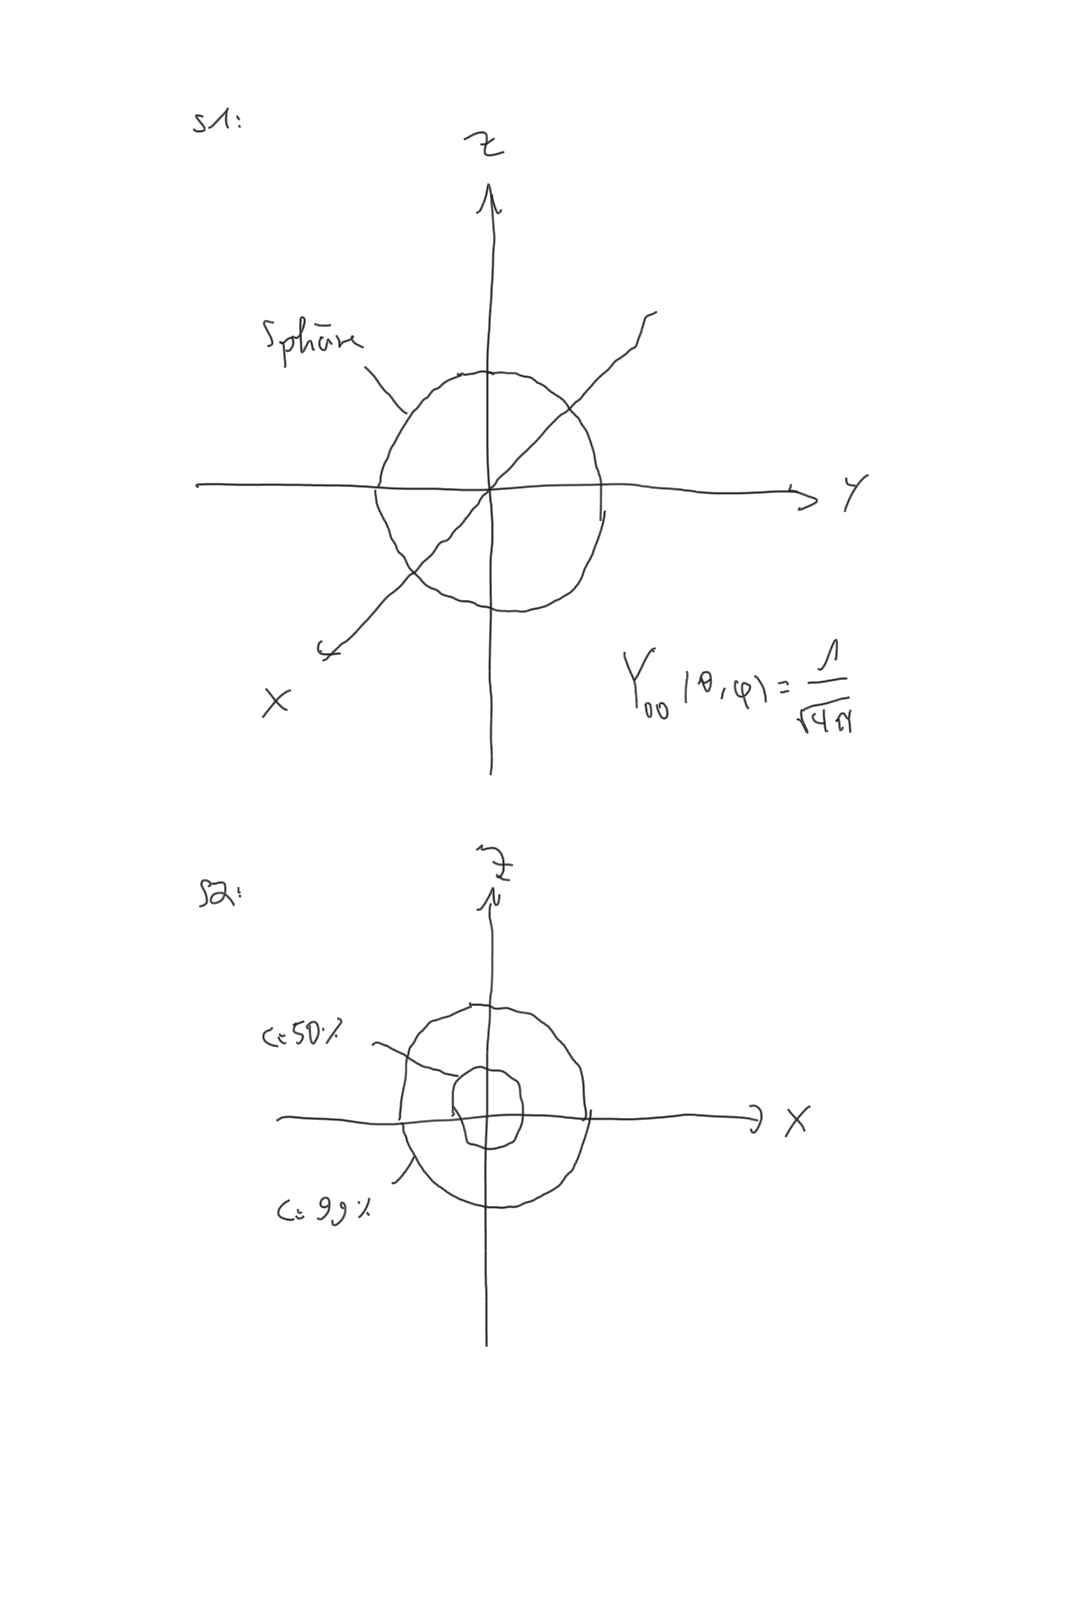
\includegraphics[width=\textwidth]{images/Skizze3a.jpg}
        \label{fig:6}
    \end{figure}

    \subsection{b)}

    \begin{align*}
        s1: P(r)\mathrm{d}r &= \int_{0}^{2\pi} \int_{0}^{\pi} \abs{\Psi(r,\theta,\varphi)}^2 r^2 \sin(\theta)\, \mathrm{d}r\, \mathrm{d}\theta\, \mathrm{d}\varphi\\
        &= \abs{R(r)}^2 r^2 \,\mathrm{d}r \int_{0}^{2\pi} \int_{0}^{\pi} \abs{Y(\theta,\varphi)}^2 \sin(\theta) \, \mathrm{d}\theta\, \mathrm{d}\varphi\\
        &= \abs{e^{-\beta\rho}}^2 r^2 \,\mathrm{d}r \int_{0}^{2\pi} \int_{0}^{\pi} \abs{\sqrt{\frac{1}{4\pi}}}^2 \sin(\theta) \, \mathrm{d}\theta\, \mathrm{d}\varphi\\
        &= \abs{e^{-\beta\rho}}^2 r^2 \,\mathrm{d}r \frac{1}{4\pi} \int_{0}^{2\pi} \left[-\cos(\theta)\right]_0^{\pi} \mathrm{d}\varphi\\
        &= \abs{e^{-\beta\rho}}^2 r^2 \,\mathrm{d}r \frac{1}{4\pi} 2\pi (1-(-1))\\
        &= e^{-2\beta\rho} r^2 \mathrm{d}r\\
        s2: P(r)\mathrm{d}r &= \int_{0}^{2\pi} \int_{0}^{\pi} \abs{\Psi(r,\theta,\varphi)}^2 r^2 \sin(\theta)\, \mathrm{d}r\, \mathrm{d}\theta\, \mathrm{d}\varphi\\
        &= \abs{R(r)}^2 r^2 \,\mathrm{d}r \int_{0}^{2\pi} \int_{0}^{\pi} \abs{Y(\theta,\varphi)}^2 \sin(\theta) \, \mathrm{d}\theta\, \mathrm{d}\varphi\\
        &= \abs{e^{-\beta\rho}\left( 1-\frac{\rho}{2} \right)}^2 r^2 \,\mathrm{d}r \int_{0}^{2\pi} \int_{0}^{\pi} \abs{\sqrt{\frac{1}{4\pi}}}^2 \sin(\theta) \, \mathrm{d}\theta\, \mathrm{d}\varphi\\
        &= \abs{e^{-\beta\rho}\left( 1-\frac{\rho}{2} \right)}^2 r^2 \,\mathrm{d}r \frac{1}{4\pi} \int_{0}^{2\pi} \left[-\cos(\theta)\right]_0^{\pi} \mathrm{d}\varphi\\
        &= \abs{e^{-\beta\rho}\left( 1-\frac{\rho}{2} \right)}^2 r^2 \,\mathrm{d}r \frac{1}{4\pi} 2\pi (1-(-1))\\
        &= e^{-2\beta\rho}\left( 1+\frac{\rho^2}{4} \right) r^2 \mathrm{d}r
    \end{align*}

    \begin{figure}[H]
        \centering
        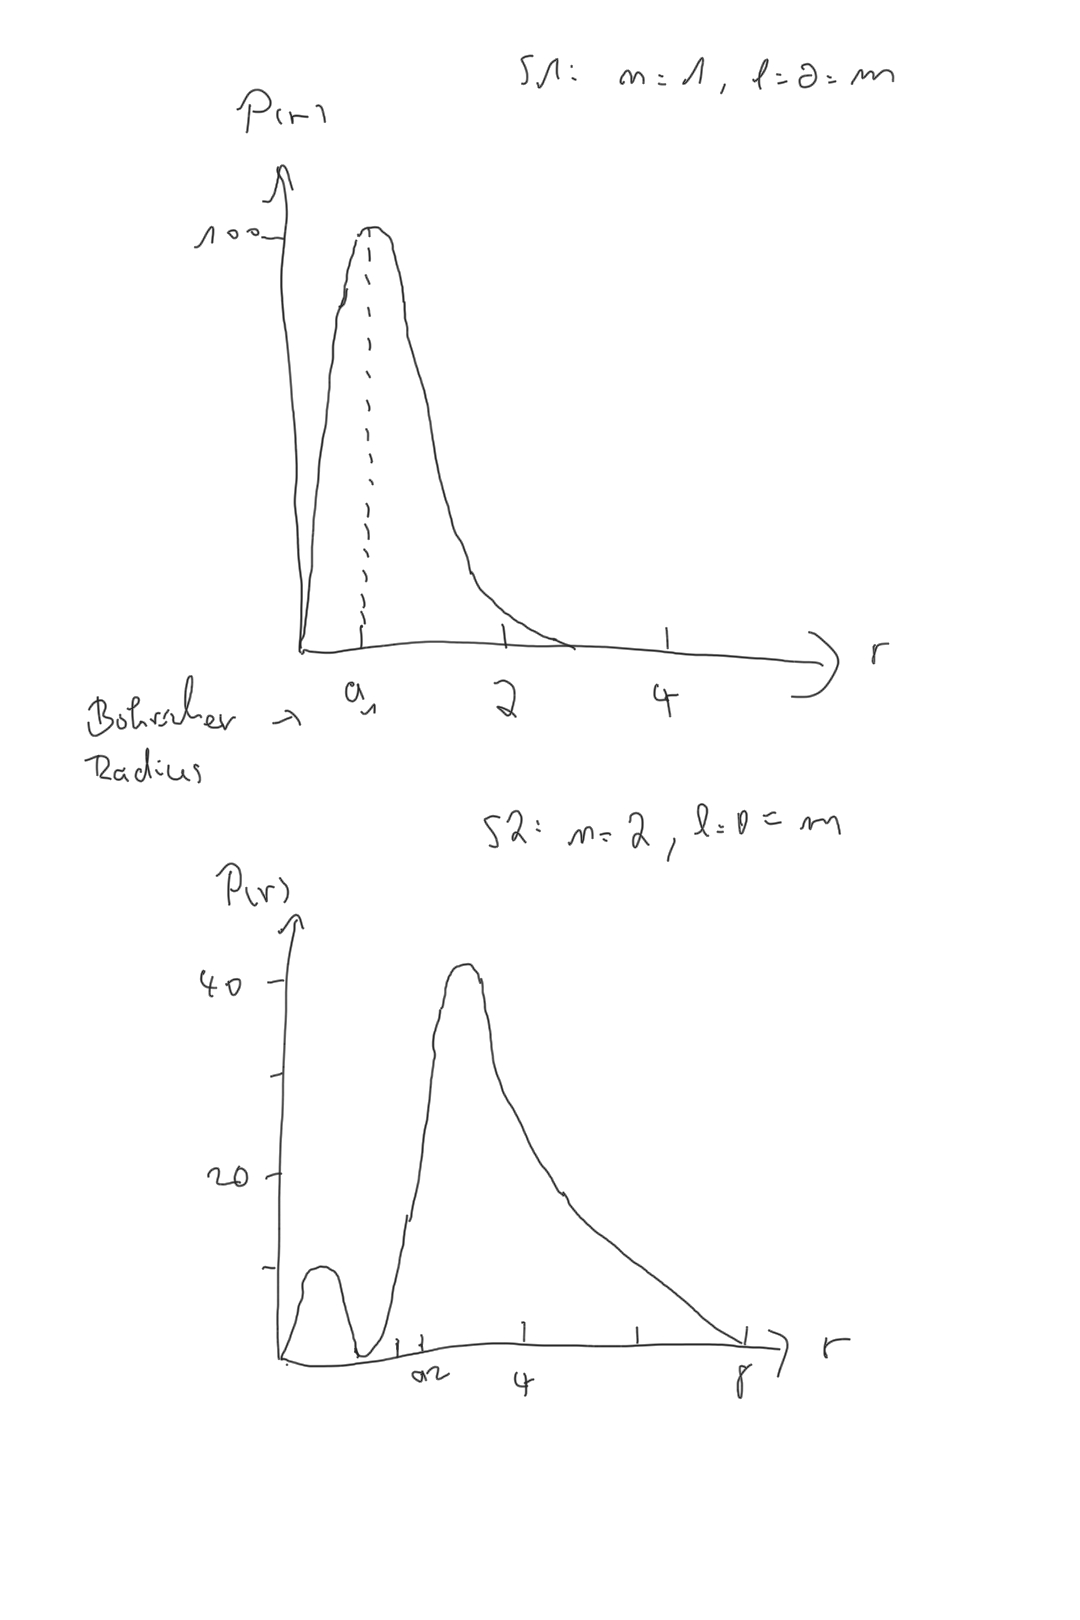
\includegraphics[width=\textwidth]{images/Skizze3b.jpg}
        \label{fig:7}
    \end{figure}

    \subsection{c)}

\section{Aufgabe 4}

    \begin{figure}[H]
        \centering
        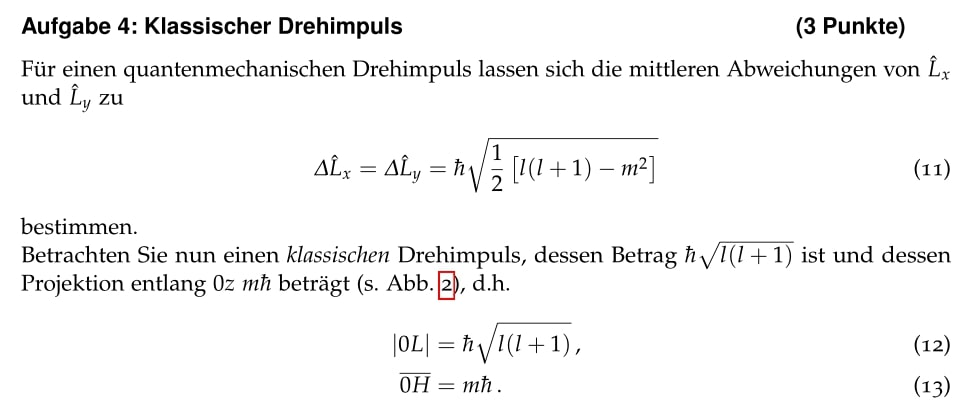
\includegraphics[width=\textwidth]{images/Aufgabe4a.jpg}
        \label{fig:8}
    \end{figure}

    \begin{figure}[H]
        \centering
        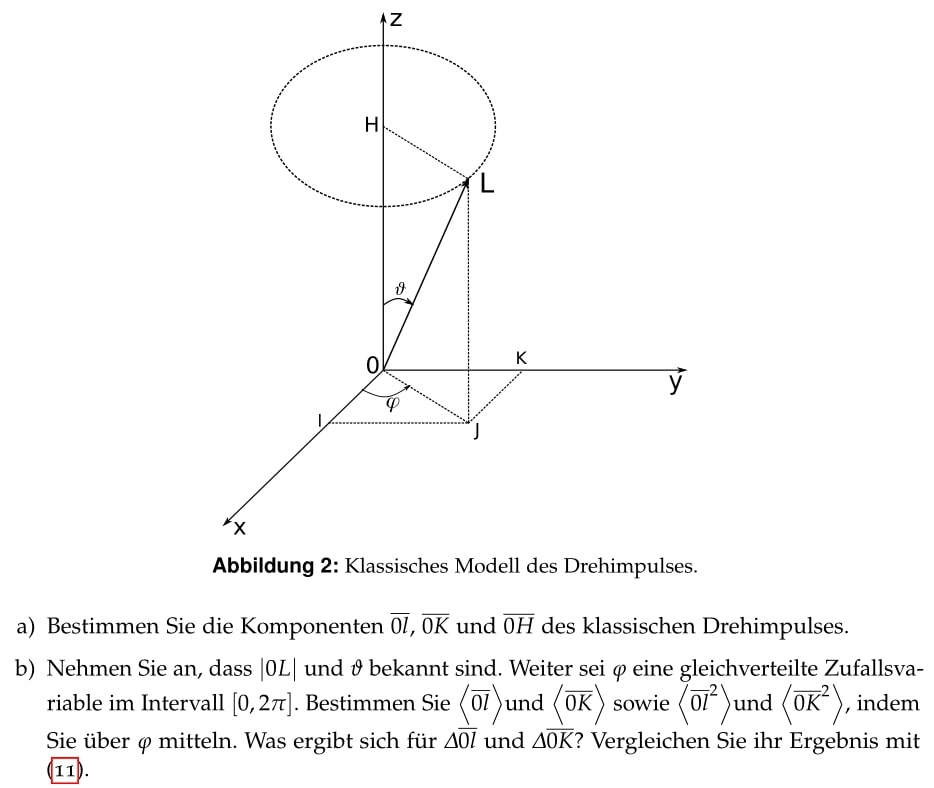
\includegraphics[width=\textwidth]{images/Aufgabe4b.jpg}
        \label{fig:9}
    \end{figure}

    \subsection{a)}

    \subsection{b)}









\end{document}